\graphicspath{{../PR2018/Figures/}}

\title{\fontsize{33}{45}{\huge Pattern Classification (EET 3035)\newline \vspace{8pt} \Large Lecture 07\vspace{-1.1cm}}}
\author{\vspace{-0.4cm}\\\normalsize{\bf Dr. Kundan Kumar}\\ PhD (IIT Kharagpur)\\
Associate Professor\\Department of ECE}
% - Give the names in the same order as the appear in the paper.
% - Use the \inst{?} command only if the authors have different
%   affiliation.

\institute[Indian Institute of Technology Kharagpur] % (optional, but mostly needed)
{

\includegraphics[height=.17\textheight]{SOAlogo.png}\\
 Faculty of Engineering (ITER)\\ S`O'A Deemed to be University, Bhubaneswar, India-751030\\
 \copyright\  2019 Kundan Kumar, All Rights Reserved\\
  \vspace{-1.1cm}}
% - Use the \inst command only if there are several affiliations.
% - Keep it simple, no one is interested in your street address.
\date{}
% To remove page number from a perticular slide
{
\setbeamertemplate{logo}{}
\makeatletter
\setbeamertemplate{footline}{
        \leavevmode%
  
  % First line.
  \hbox{%
  \begin{beamercolorbox}[wd=.2\paperwidth,ht=\beamer@decolines@lineup,dp=0pt]{}%
  \end{beamercolorbox}%
  \begin{beamercolorbox}[wd=.8\paperwidth,ht=\beamer@decolines@lineup,dp=0pt]{lineup}%
  \end{beamercolorbox}%
  } %
  % Second line.
  \hbox{%
  \begin{beamercolorbox}[wd=\paperwidth,ht=\beamer@decolines@linemid,dp=0pt]{linemid}%
  \end{beamercolorbox}%
  } %
  % Third line.
  \hbox{%
  \begin{beamercolorbox}[wd=.1\paperwidth,ht=\beamer@decolines@linebottom,dp=0pt]{}%
  \end{beamercolorbox}%
  \begin{beamercolorbox}[wd=.9\paperwidth,ht=\beamer@decolines@linebottom,dp=0pt]{linebottom}%
  \end{beamercolorbox}%
  }%
        }
\makeatother
\begin{frame}
\titlepage
\end{frame}
}


\section{Neural Network}
\subsection{}

\begin{frame}{}
\begin{variableblock}{\centering \Large \textbf{\vspace{4pt}\newline Artificial Neural Networks\vspace{4pt}}}{bg=slidecolor,fg=white}{bg=slidecolor,fg=white}
\end{variableblock}
\end{frame}

\begin{frame}{What is Neural Network?}
\begin{itemize}
\item \textit{\color{slidecolor}Neural Networks} are networks of neurons, for example, as found in real (i.e. biological) brains
\begin{figure}
\includegraphics[scale=0.18]{BioNeuron.jpg}
\end{figure}
\item \textit{\color{slidecolor}Artificial neurons} are crude approximation of the neurons found in real brains.
\begin{figure}
\includegraphics[scale=0.18]{ArtNeuron.jpeg}
\end{figure}
\end{itemize}
\end{frame}

\begin{frame}{Artificial Neural Network (ANNs)}
\begin{itemize}
\item Artificial Neural Network (ANNs) are network of Artificial Neurons and hence constitute crude approximation to parts of real brains.
\begin{figure}
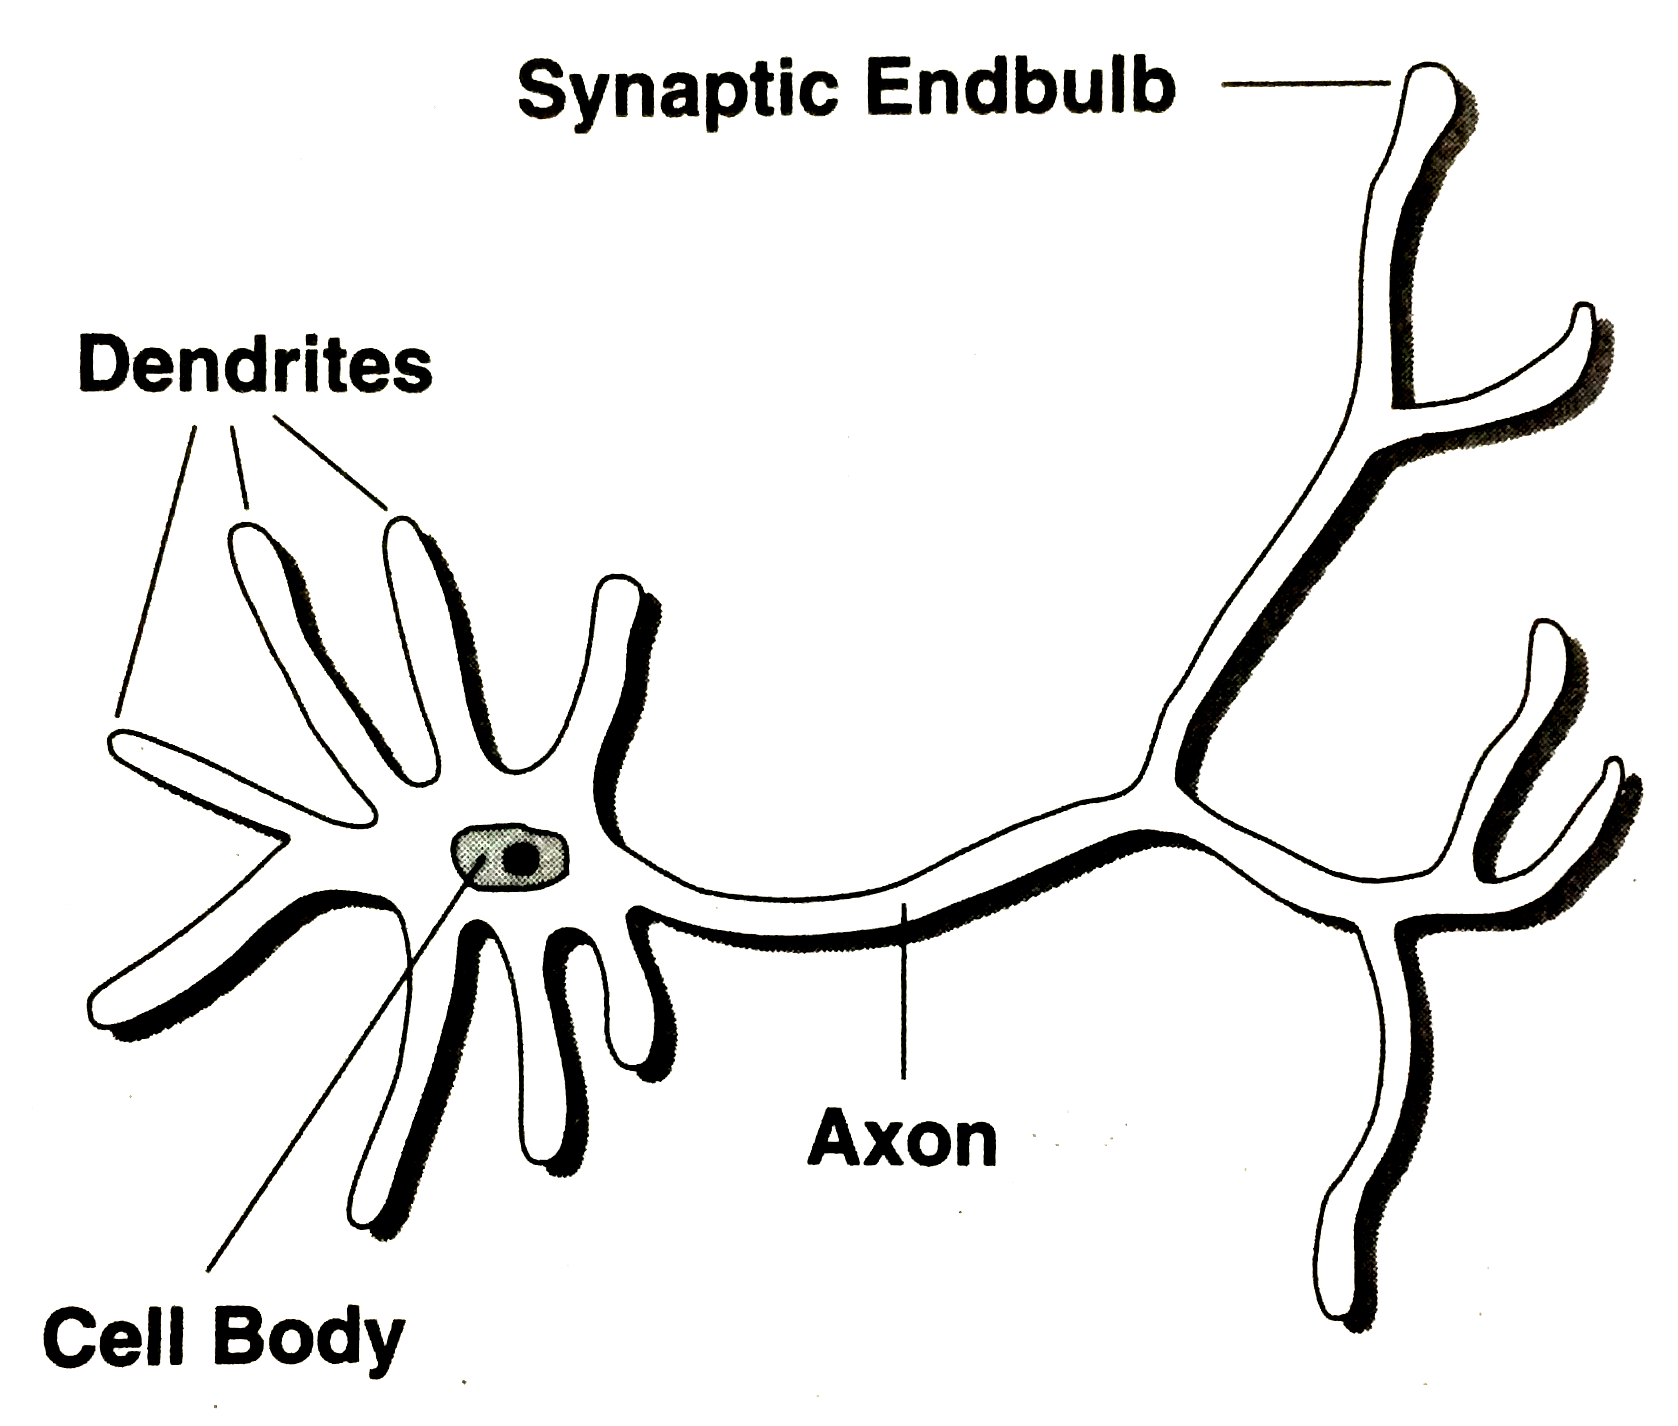
\includegraphics[scale=0.1]{ann02.JPG}
\end{figure}
\end{itemize}
\end{frame}

\begin{frame}{Why are Artificial Neural Networks worth studying?}
\begin{itemize}
\item They are extremely powerful computational devices
\item Massive parallelism makes them very efficient
\item They can learn and generalize from training data -- so there is no need for enormous feats of programming
\end{itemize}
\end{frame}

\begin{frame}{Neural Network Applications}
\begin{itemize}
\item Brain Modeling
\begin{itemize}
\item Aid our understanding of how the brain works, how behavior emerges from the interaction of networks of neurons, what needs to “get fixed” in brain
damaged patients
\end{itemize}
\item Real world application
\begin{itemize}
\item Financial modeling -- predicting the stock market
\item Time series prediction -- climate, weather, seizures
\item Computer games -- intelligent agents, chess, backgammon
\item Robotics -- autonomous adaptable robots
\item Pattern recognition -- speech recognition, seismic activity, sonar signals
\item Data analysis -- data compression, data mining
\item Bioinformatics -- DNA sequencing, alignment
\end{itemize}
\end{itemize}
\end{frame}

\begin{frame}{Brain vs. Computers}
\begin{footnotesize}
\begin{itemize}
\item \textit{\color{slidecolor}Processing elements:} There are $10^{14}$ synapses in the brain, compared with $10^8$ transistors in the computer
\item \textit{\color{slidecolor}Processing speed:} 100 Hz for the brain compared to $10^9$ Hz for the computer
\item \textit{\color{slidecolor}Style of computation:} The brain computes in parallel and distributed mode, whereas the computer mostly serially and centralized.
\item \textit{\color{slidecolor}Fault tolerant:} The brain is fault tolerant, whereas the computer is not. 
\item \textit{\color{slidecolor}Adaptive:} The brain learns fast, whereas the computer doesn't even compare with an infant's learning capabilities
\item \textit{\color{slidecolor}Intelligence and consciousness:} The brain is highly intelligent and
conscious, whereas the computer shows lack of intelligence
\item \textit{\color{slidecolor}Evolution:} The brains have been evolving for tens of millions of years,
computers have been evolving for decades.
\end{itemize}
\end{footnotesize}
\end{frame}

\begin{frame}{Decision Boundaries for AND and OR}
\begin{figure}
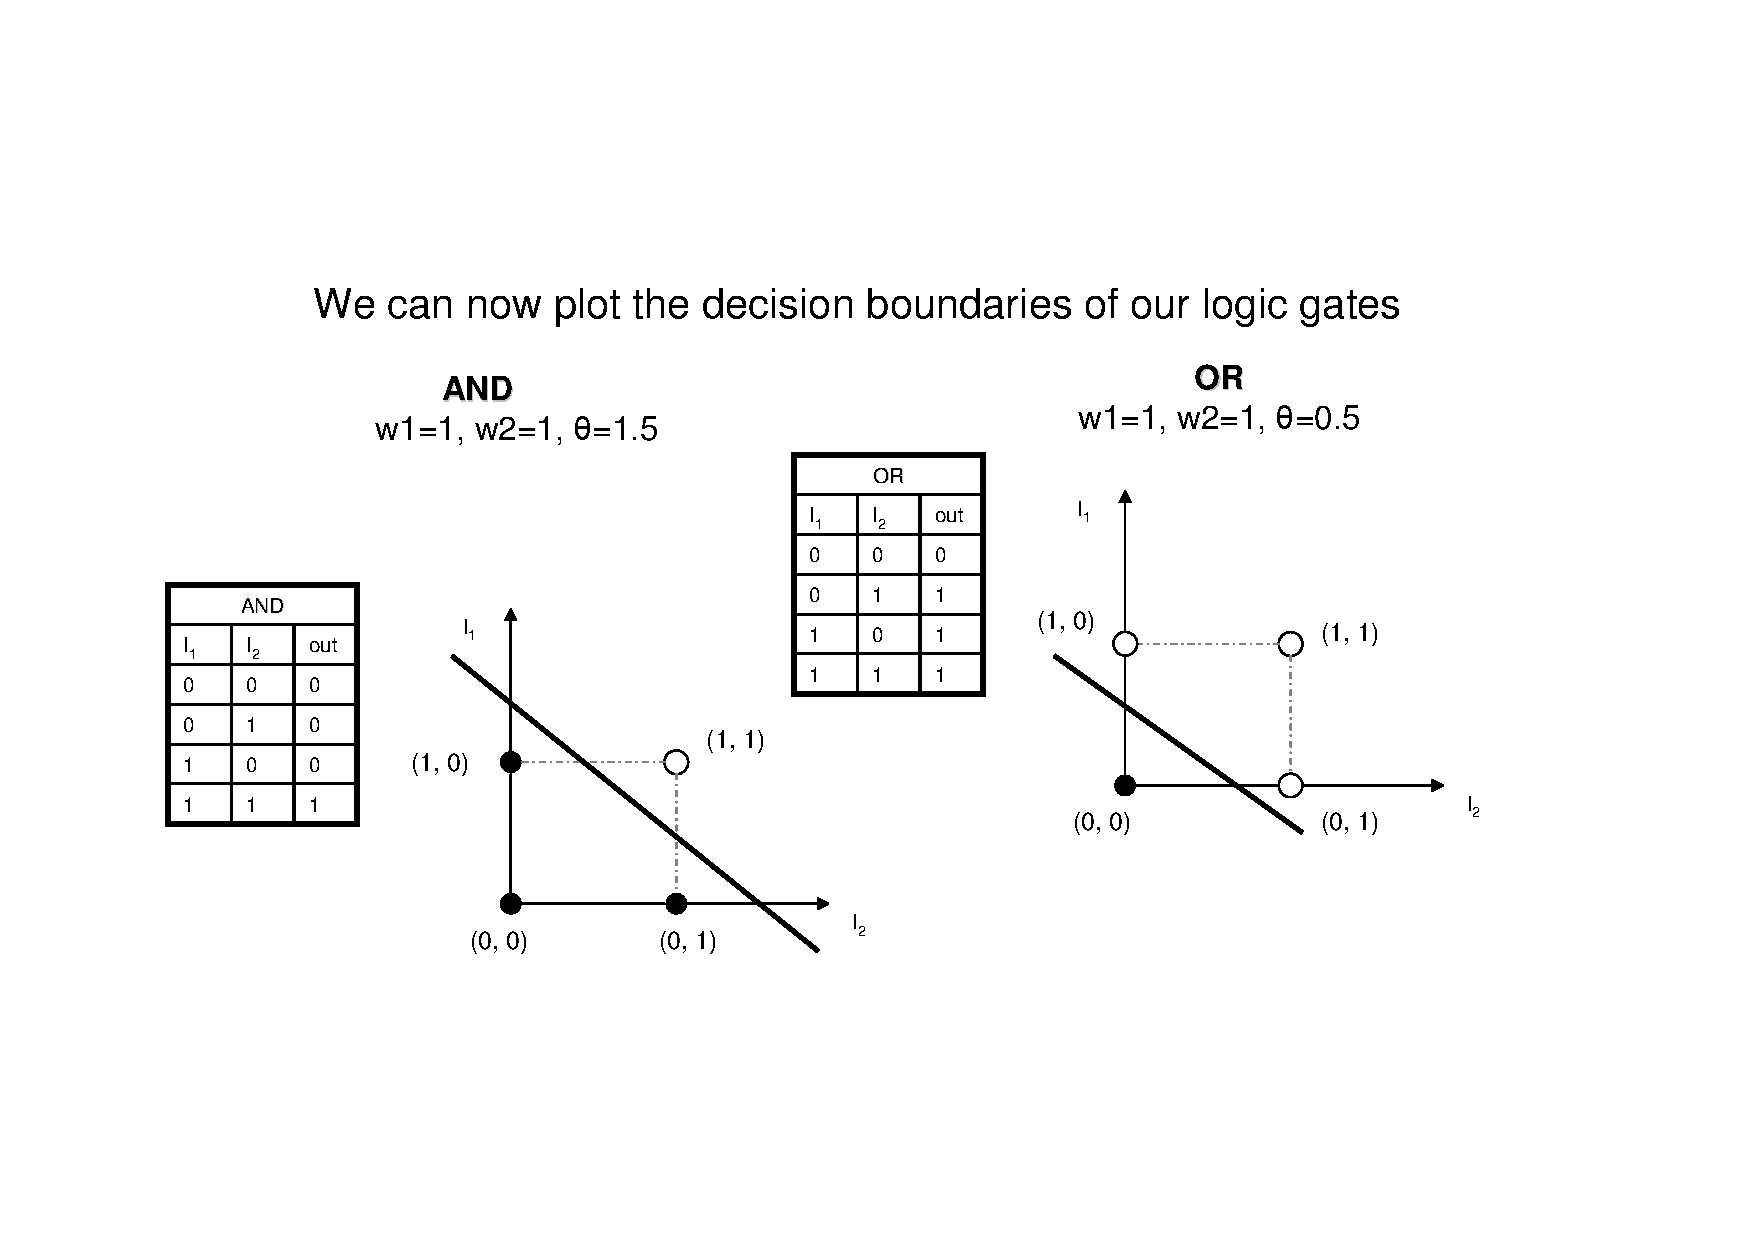
\includegraphics[scale=0.45]{ann01}
\end{figure}
\end{frame}

\begin{frame}{Types of Activation/Transfer Function}
\begin{itemize}
\item Threshold Function
\item Piecewise-Linear Function
\item Sigmoid Function
\end{itemize}
\end{frame}

\begin{frame}{Basic Neural Model in A Feedforward Network}
\begin{adjustwidth}{-1cm}{-1cm}
\begin{columns}
\begin{column}{5cm}
\begin{itemize}
\item Input $x_i$ arrive through pre-synaptic connections
\item Synaptic efficacy is modeled using real weight $w_i$
\item The response of the neuron is a nonlinear function $f$ of its weighted inputs.
\end{itemize}
\end{column}
\begin{column}{7cm}
\begin{figure}
\includegraphics[scale=0.4]{BasicNN}
\end{figure}
\end{column}
\end{columns}
\end{adjustwidth}
\end{frame}

\begin{frame}{Input to Neurons}
\begin{itemize}
\item Arise from other neurons or from outside the network
\item Nodes whose inputs arise outside the network are called input nodes and simply copy values
\item An input may excite or inhibit the response of the neuron to which it is applied, depending upon the weight of the connection.
\end{itemize}
\end{frame}

\begin{frame}{A single neuron what can do?}
\begin{itemize}
\item This is basically a special case of the neuron-like processing unit.
\begin{figure}
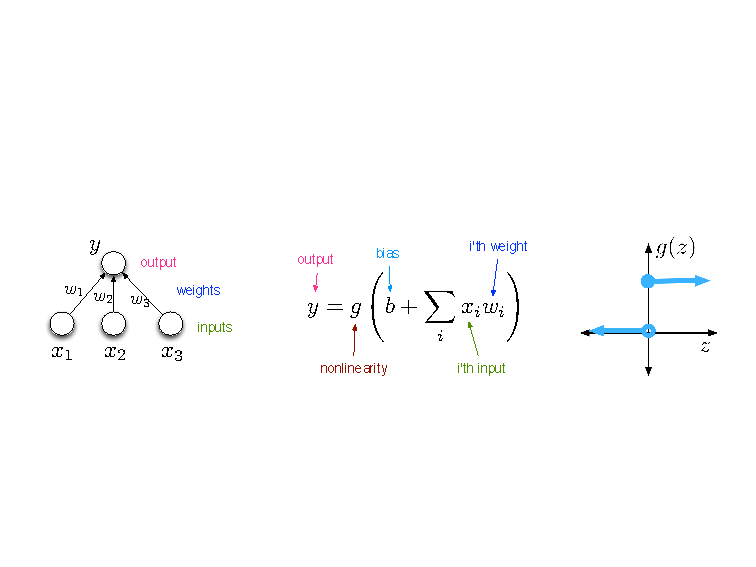
\includegraphics[scale=0.9]{ann03.pdf}
\end{figure}
\end{itemize}
\end{frame}

\begin{frame}{An abstract mathematical model of a neuron}
\begin{itemize}
\item McCulloch and Pitts given a first attempt to form an abstract mathematical model of a neuron in 1943.
\item The model 
\begin{itemize}
\setlength{\itemsep}{5pt}
\item receives a finite number of inputs $x_1,x_2,\ldots,x_M$
\item computes the weighted sum $s = \sum\nolimits_{i = 1}^M {{w_i}{x_i}}$ using the weights $w_1,w_2,\ldots,w_M$
\item thresholds $s$ and output 0 or 1 depending on whether the weighted sum is less than or greater than a given threshold value $T$.
\end{itemize}
\end{itemize}
\end{frame}

\begin{frame}{McCulloch-Pitts model of the neuron}
\begin{figure}
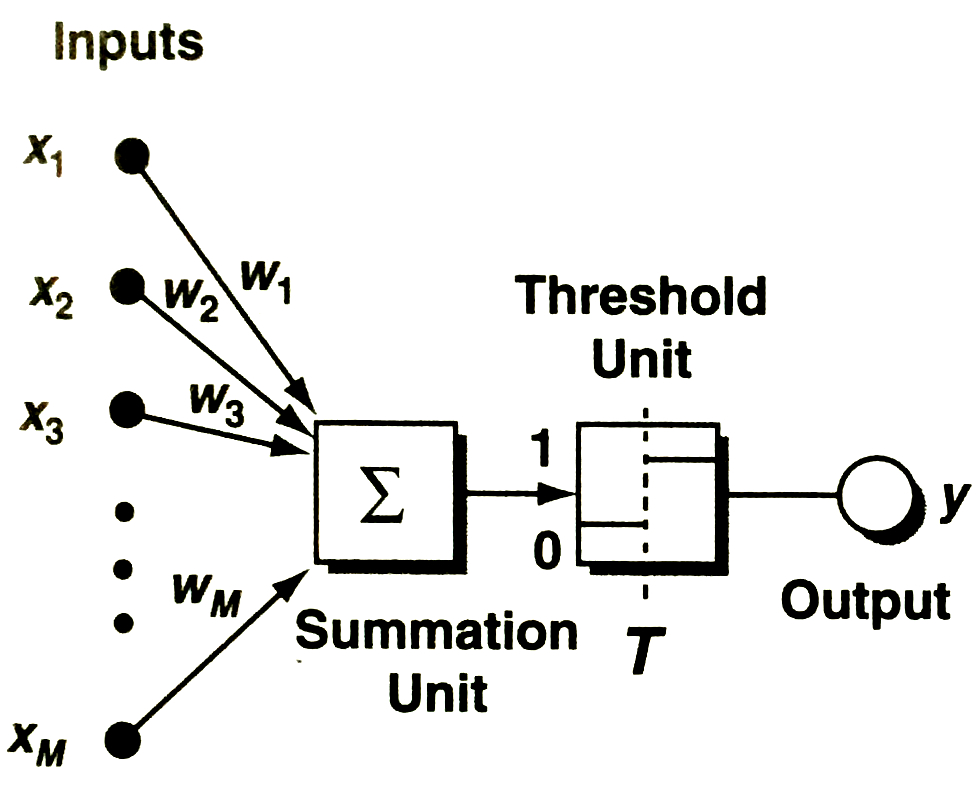
\includegraphics[scale=0.15]{ann04.JPG}~~~~~~~
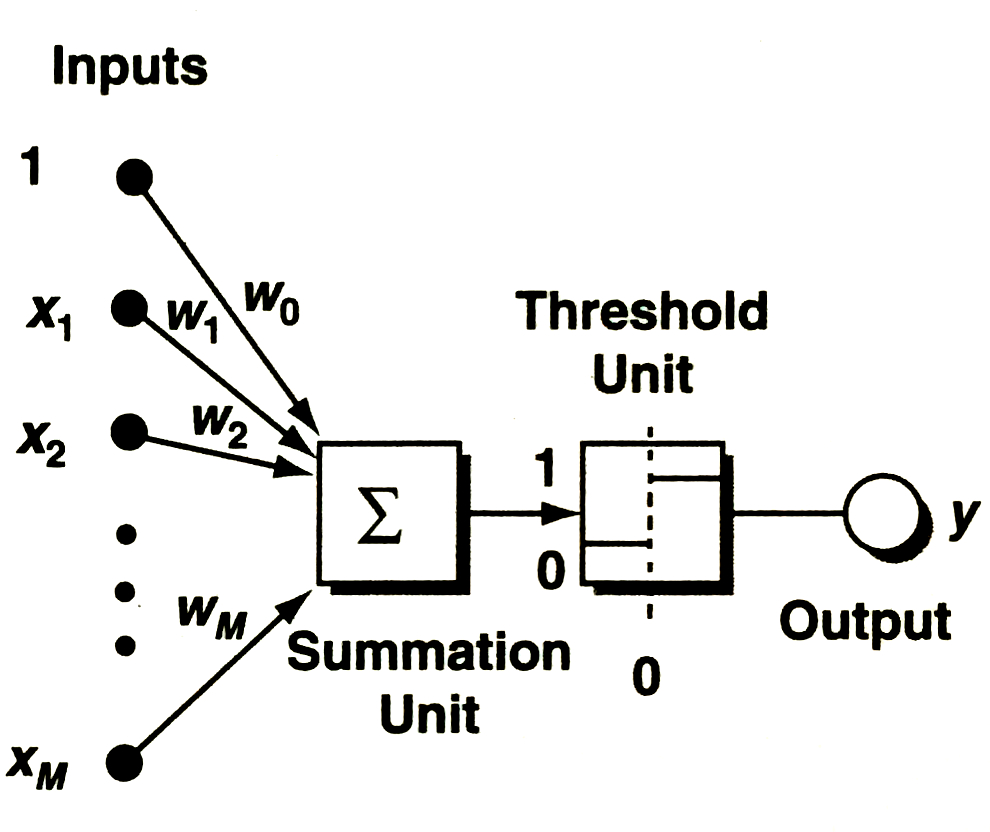
\includegraphics[scale=0.15]{ann05.JPG}
\end{figure}
\end{frame}


\begin{frame}{McCulloch-Pitts model of the neuron}
\begin{itemize}
\item Summation is indicated by sigma and thresholding is shown by a small graph of the function.
\item The combination of summation and thresholding is called a \textit{\color{slidecolor}node} in an artificial neural network.
\item Nodes are denoted by open circles in the diagrams of neural networks.
\item Node inputs with positive weights are called \textit{\color{slidecolor}excitory} and node inputs with negative weights are called \textit{\color{slidecolor}inhibitory}.
\end{itemize}
\end{frame}

\begin{frame}{McCulloch-Pitts model of the neuron}
\begin{itemize}
\item The output of the model neuron is 1 if
\begin{equation}
w_1x_1+w_2x_2+\cdots+w_Mx_M>T\nonumber
\end{equation}
and 0 otherwise.
\item For convenience we can write
\begin{equation}
D=w_1x_1+w_2x_2+\cdots+w_Mx_M\nonumber
\end{equation}
where $w_0=-T$ and $x_0=1$
\item Output 1 if $D>0$ and output 0 if $D\leq 0$.
\item Weight $w_0$ is called the bias weight.
\end{itemize}
\end{frame}

\begin{frame}{McCulloch-Pitts model of the neuron with bias}
\begin{figure}
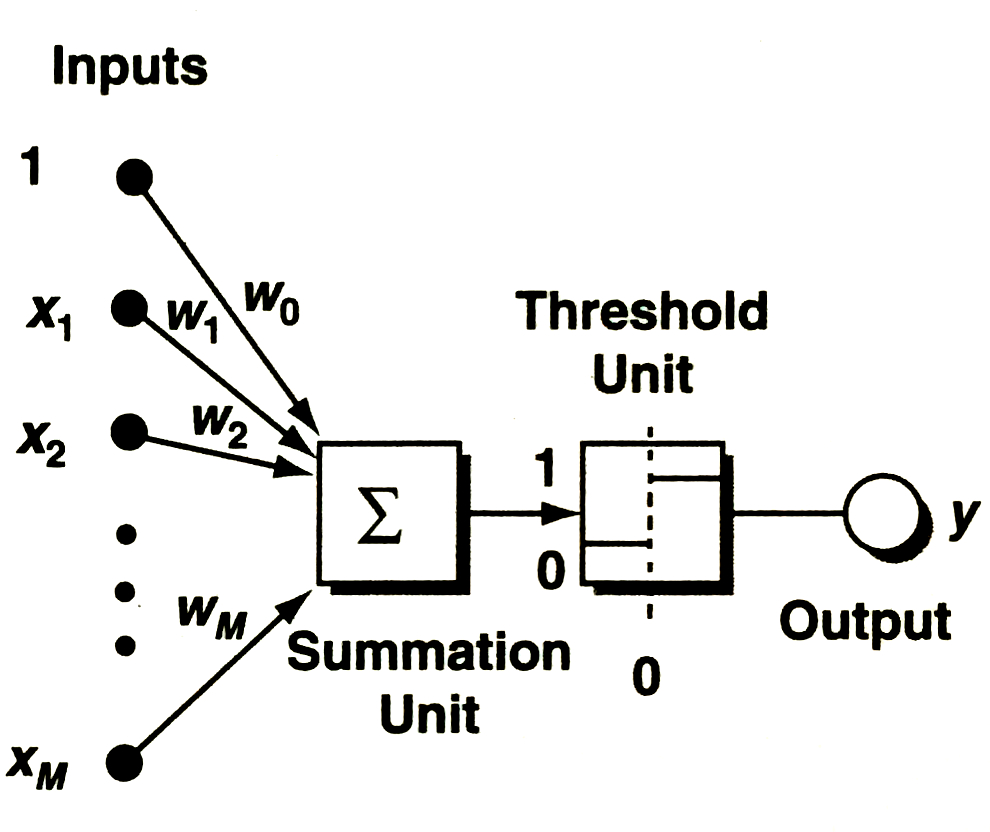
\includegraphics[scale=0.15]{ann05.JPG}
\end{figure}
\end{frame}


\begin{frame}{Nets without Hidden Layers}
\begin{itemize}
\item \textit{\color{slidecolor}Two-layer nets}: a layer of input nodes that are directly connected to the layer of output nodes.
\begin{figure}
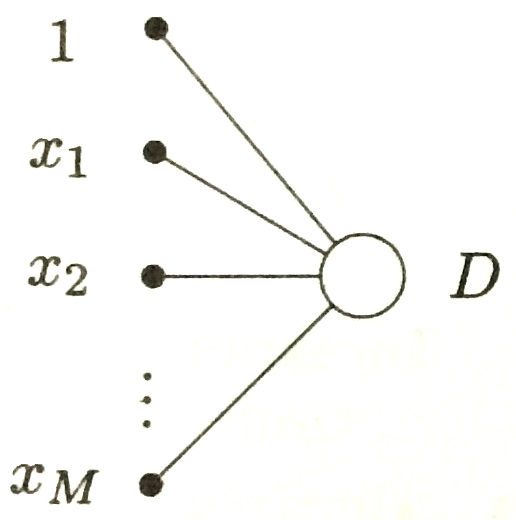
\includegraphics[scale=0.13]{ann06.JPG}~~~~~~~~~
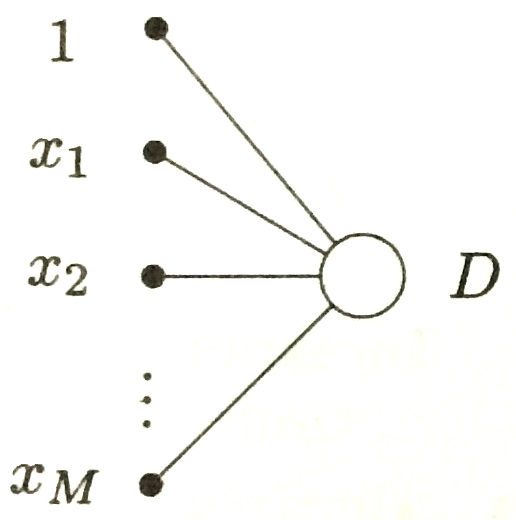
\includegraphics[scale=0.13]{ann06.JPG}
\caption{(a) A two-layer neural net with one output node. The weight connecting input $x_i$ with the output $D$ is $w_i$. (b) A two-layer network net with multiple output nodes. The weight connecting input $x_i$ with output $D_j$ is $w_j$}
\end{figure}
\item The layers of nodes between the input and output layers are called \textit{\color{slidecolor} hidden layers}.
\end{itemize}
\end{frame}

\begin{frame}{}
\begin{itemize}
\item \textit{\color{slidecolor}Training:} A difficult aspect of using a neural net is finding weights that solve problems with acceptable performance.
\begin{itemize}
\item Back-propagation algorithm
\end{itemize}
\item A variety of pattern can be classified using a two-layer net.
\end{itemize}
\end{frame}

\begin{frame}{Example: Logical AND function}
\begin{figure}
\includegraphics[scale=0.065]{ann09.JPG}
\end{figure}
\begin{figure}
\includegraphics[scale=0.11]{ann10.JPG}
\caption{(a) The separating line $-1.5+x_1+x_2=0$ for the logical AND pattern. (b) A two-layer net implementing the logical AND}
\end{figure}
\end{frame}

\begin{frame}{Example: Logical OR function}
\begin{figure}
\includegraphics[scale=0.1]{ann11.JPG}
\end{figure}
\begin{figure}
\includegraphics[scale=0.12]{ann12.JPG}
\caption{(a) The separating line $-0.5+x_1+x_2=0$ for the logical OR pattern.}
\end{figure}
\end{frame}

\begin{frame}{Example: Logical XOR function}
\begin{figure}
\includegraphics[scale=0.15]{ann13.JPG}
\end{figure}
\begin{figure}
\includegraphics[scale=0.12]{ann14.JPG}
\caption{(a) no single separating line exists for the exclusive OR pattern}
\end{figure}
\end{frame}

\begin{frame}{The Sequential MSE Algorithm}
\begin{itemize}
\item The goal of the minimum squared error procedure is to find the values of the weights $w_0,w_1,\ldots,w_M$ that minimize the criterion function
\begin{equation}
E = \frac{1}{2}\sum\limits_{p = 1}^N {{{({D_p} - {d_p})}^2}} \nonumber
\end{equation}
where
$D_p=w_0+w_1x_{p1}+\ldots+w_Mx_{pM}$, $d_p$ is the desired output for sample $p$, and $x_{p1},\ldots,x_{pM}$ are the feature values of sample.
\end{itemize}
\end{frame}

\begin{frame}{Steepest algorithm}
\begin{itemize}
\item[1.] Pick a starting guess $w_1,w_2,\ldots,w_M$ and choose a positive constant $c$.
\item[2.] Compute the partial derivatives $\partial F/\partial w_i$, for $i=1,2,\ldots,M$. Replace $w_i$ by $w_i-c\partial F/\partial w_i$ for $i=1,2,\ldots,M$.
\item[3.] Repeat step 2 until $w_1,w_2,\ldots,w_M$ cease to change significantly.
\end{itemize}
\end{frame}

\begin{frame}{The sequential MSE algorithm for Multiple outputs}
\begin{itemize}
\item[1.] Pick starting weight $w_0,\ldots,w_M$ and choose a positive constant $c$.
\item[2.] Present samples 1 through $N$ repeatedly to the classifier, cycling back to sample 1 after sample $N$ is encountered. For each sample, compute
\begin{equation}
D_j=w_{0j}+w_{1j}x_1+\ldots+w_{Mj}x_M\nonumber
\end{equation}
for nodes $j=1,\ldots,M_1$
\item[3.] Replace $w_{ij}$ by $w_{ij}-c(D_j-d_j)x_i$ for all $i$
\item[4.] Repeat steps 2 and 3 until the weights cease to change significantly.
\end{itemize}
Algorithm usually works well if the classes are well separated.
\end{frame}

\begin{frame}{Multilayer Perceptron}
\begin{itemize}
\item Mutlilayer network has $K+1$ layers of nodes, denoted $0,1,\ldots,K$.
\item $x_i^{(k)}: $ the output of the $i^{th}$ node in $k^{th}$ layer
\begin{itemize}
\item This is the value obtained after computing the weighted sum of the inputs and applying the threshold or other function
\end{itemize}
\item The layer of input nodes has index $k=0$ and is called \textit{\color{slidecolor}input layer/retina}.
\item The nodes in layer $K$ are called the \textit{\color{slidecolor}output nodes}.
\item Those in layer 1 through $K-1$ are called the \textit{\color{slidecolor}hidden nodes}
\end{itemize}
\end{frame}

\begin{frame}{Nets with Hidden Layers}
\begin{figure}
\includegraphics[scale=0.13]{ann16.JPG}
\caption{A four-layer neural net. The weight connecting node $x_i^{(k-1)}$ with node $x_j^{(k)}$ is $w_{ij}^{(k)}$.}
\end{figure}
\end{frame}

\begin{frame}{Example: Exclusive OR }
\begin{figure}
\includegraphics[scale=0.11]{ann17.JPG}
\caption{The implementation of the exclusive OR mapping}
\end{figure}
\begin{equation}
-0.5+x_1+x_2\geq 0~~~{\rm AND}~~~1.5-x_1-x_2\geq0\nonumber
\end{equation}
\end{frame}

\section{Activation Functions}
\subsection{}
\begin{frame}{Activation Function: Sigmoidal}
\begin{itemize}
\item It is also known as Logistic Activation Function.
\item It takes a real-valued number and squashes it into a range between 0 and 1. 
\item It is also used in the output layer where our end goal is to predict probability. 
\item Mathematically it is represented as
\begin{equation}
R(s) = \frac{1}{{1 + {e^{ - s}}}} \nonumber
\end{equation}
\begin{figure}[h]
\centering
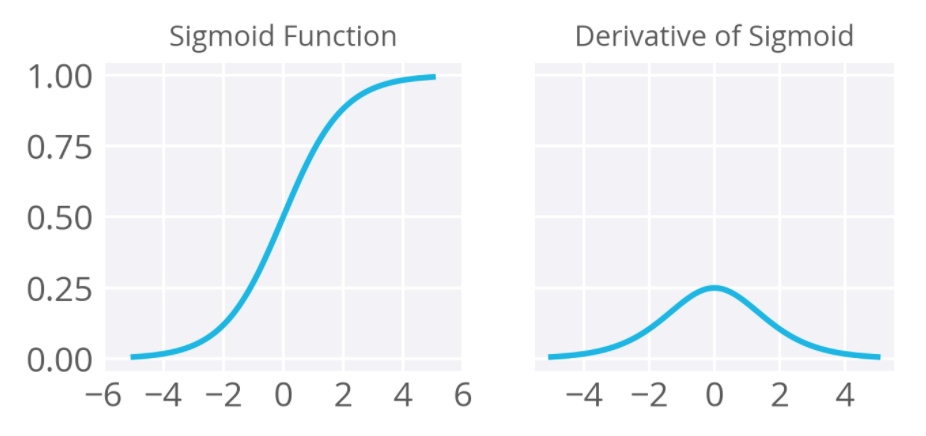
\includegraphics[scale=0.2]{AF001}
\end{figure}
\end{itemize}
\end{frame}


\section{References}
\subsection{}
\begin{frame}[allowframebreaks]{References}
\linespread{1}
\footnotesize
\printbibliography[heading=none]
\end{frame}
{
\nocite{Daugman1985}\nocite{Petkov1995}\nocite{Petkov1997}\nocite{Kruizinga1999}\nocite{Grigorescu2002}\nocite{Petkov2003}\nocite{Grigorescu2003}\nocite{Jain1991}
\setbeamertemplate{logo}{}
\makeatletter
\setbeamertemplate{footline}{
        \leavevmode%
  
  % First line.
  \hbox{%
  \begin{beamercolorbox}[wd=.2\paperwidth,ht=\beamer@decolines@lineup,dp=0pt]{}%
  \end{beamercolorbox}%
  \begin{beamercolorbox}[wd=.8\paperwidth,ht=\beamer@decolines@lineup,dp=0pt]{lineup}%
  \end{beamercolorbox}%
  } %
  % Second line.
  \hbox{%
  \begin{beamercolorbox}[wd=\paperwidth,ht=\beamer@decolines@linemid,dp=0pt]{linemid}%
  \end{beamercolorbox}%
  } %
  % Third line.
  \hbox{%
  \begin{beamercolorbox}[wd=.1\paperwidth,ht=\beamer@decolines@linebottom,dp=0pt]{}%
  \end{beamercolorbox}%
  \begin{beamercolorbox}[wd=.9\paperwidth,ht=\beamer@decolines@linebottom,dp=0pt]{linebottom}%
  \end{beamercolorbox}%
  }%
        }
\makeatother

\begin{frame}
\centering

\includegraphics[width=0.4\paperwidth]{queries.jpg}\\

\includegraphics[width=0.5\paperwidth]{thank_you.png}
\end{frame}
}